\documentclass{standalone}
\usepackage{tikz}
\usetikzlibrary{patterns, positioning}

\begin{document}
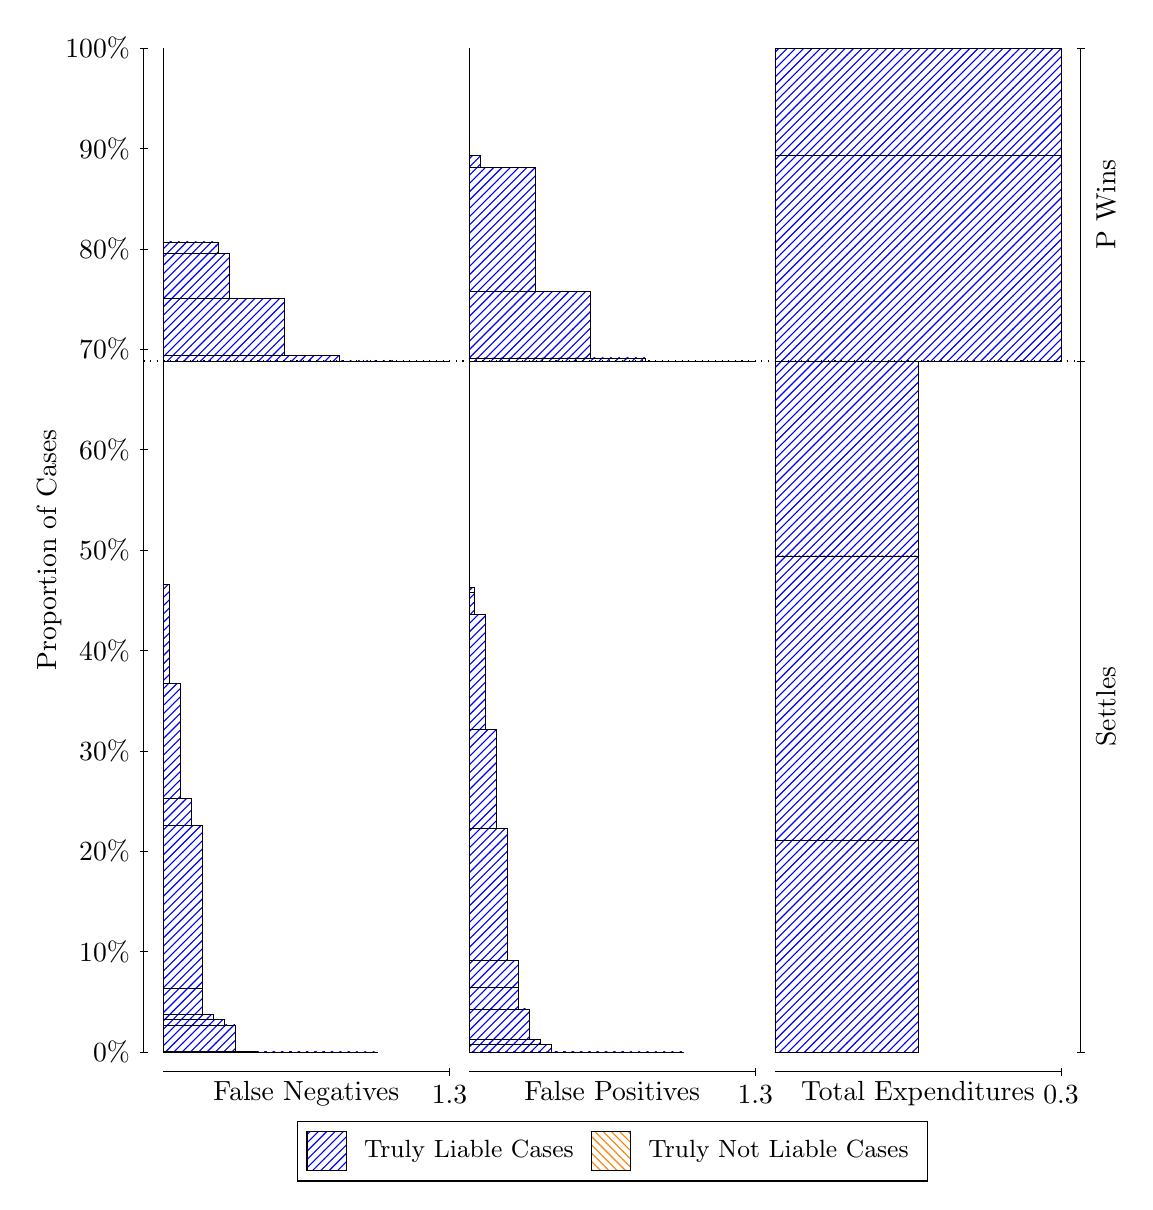
\begin{tikzpicture}
\draw[black, very thin] (1.5,1.75) -- (1.5,14.5);
\node[rotate=90, anchor=center] at (0.3, 8.125) {Proportion of Cases};
\draw[black, very thin] (1.45,1.75) -- (1.55,1.75);
\node[anchor=east] at (1.45, 1.75) {0\%};
\draw[black, very thin] (1.45,3.025) -- (1.55,3.025);
\node[anchor=east] at (1.45, 3.025) {10\%};
\draw[black, very thin] (1.45,4.3) -- (1.55,4.3);
\node[anchor=east] at (1.45, 4.3) {20\%};
\draw[black, very thin] (1.45,5.575) -- (1.55,5.575);
\node[anchor=east] at (1.45, 5.575) {30\%};
\draw[black, very thin] (1.45,6.85) -- (1.55,6.85);
\node[anchor=east] at (1.45, 6.85) {40\%};
\draw[black, very thin] (1.45,8.125) -- (1.55,8.125);
\node[anchor=east] at (1.45, 8.125) {50\%};
\draw[black, very thin] (1.45,9.4) -- (1.55,9.4);
\node[anchor=east] at (1.45, 9.4) {60\%};
\draw[black, very thin] (1.45,10.675) -- (1.55,10.675);
\node[anchor=east] at (1.45, 10.675) {70\%};
\draw[black, very thin] (1.45,11.95) -- (1.55,11.95);
\node[anchor=east] at (1.45, 11.95) {80\%};
\draw[black, very thin] (1.45,13.225) -- (1.55,13.225);
\node[anchor=east] at (1.45, 13.225) {90\%};
\draw[black, very thin] (1.45,14.5) -- (1.55,14.5);
\node[anchor=east] at (1.45, 14.5) {100\%};

\draw[black, very thin] (13.4,1.75) -- (13.4,14.5);
\draw[black, very thin] (13.35,1.75) -- (13.45,1.75);
\node[anchor=west] at (13.35, 1.75) {};
\draw[black, very thin] (13.35,10.525) -- (13.45,10.525);
\node[anchor=west] at (13.35, 10.525) {};
\draw[black, very thin] (13.35,14.5) -- (13.45,14.5);
\node[anchor=west] at (13.35, 14.5) {};

\draw[black, very thin, pattern color=blue, pattern=north east lines] (1.75,1.75) rectangle (4.475,1.75);
\draw[black, very thin, pattern color=blue, pattern=north east lines] (1.75,1.75) rectangle (4.1955,1.75);
\draw[black, very thin, pattern color=blue, pattern=north east lines] (1.75,1.75) rectangle (3.916,1.75);
\draw[black, very thin, pattern color=blue, pattern=north east lines] (1.75,1.75) rectangle (3.7763,1.75);
\draw[black, very thin, pattern color=blue, pattern=north east lines] (1.75,1.75) rectangle (3.6365,1.75);
\draw[black, very thin, pattern color=blue, pattern=north east lines] (1.75,1.75) rectangle (3.4968,1.75);
\draw[black, very thin, pattern color=blue, pattern=north east lines] (1.75,1.75) rectangle (3.3571,1.7508);
\draw[black, very thin, pattern color=blue, pattern=north east lines] (1.75,1.7508) rectangle (3.2173,1.7508);
\draw[black, very thin, pattern color=blue, pattern=north east lines] (1.75,1.7508) rectangle (3.0776,1.7508);
\draw[black, very thin, pattern color=blue, pattern=north east lines] (1.75,1.7508) rectangle (2.9378,1.7537);
\draw[black, very thin, pattern color=blue, pattern=north east lines] (1.75,1.7537) rectangle (2.7981,1.7575);
\draw[black, very thin, pattern color=blue, pattern=north east lines] (1.75,1.7575) rectangle (2.6583,2.0954);
\draw[black, very thin, pattern color=blue, pattern=north east lines] (1.75,2.0954) rectangle (2.5186,2.1614);
\draw[black, very thin, pattern color=blue, pattern=north east lines] (1.75,2.1614) rectangle (2.3788,2.2252);
\draw[black, very thin, pattern color=blue, pattern=north east lines] (1.75,2.2252) rectangle (2.2391,2.5622);
\draw[black, very thin, pattern color=blue, pattern=north east lines] (1.75,2.5622) rectangle (2.2391,4.6279);
\draw[black, very thin, pattern color=blue, pattern=north east lines] (1.75,4.6279) rectangle (2.0994,4.9658);
\draw[black, very thin, pattern color=blue, pattern=north east lines] (1.75,4.9658) rectangle (1.9596,6.4281);
\draw[black, very thin, pattern color=blue, pattern=north east lines] (1.75,6.4281) rectangle (1.8199,7.6837);
\draw[black, very thin, pattern color=orange, pattern=north west lines] (1.75,7.6837) rectangle (1.75,7.6837);
\draw[black, very thin, pattern color=blue, pattern=north east lines] (1.75,7.6837) rectangle (1.75,10.525);
\draw[black, very thin, pattern color=blue, pattern=north east lines] (1.75,10.525) rectangle (5.3833,10.525);
\draw[black, very thin, pattern color=blue, pattern=north east lines] (1.75,10.525) rectangle (4.6846,10.526);
\draw[black, very thin, pattern color=blue, pattern=north east lines] (1.75,10.526) rectangle (3.9859,10.597);
\draw[black, very thin, pattern color=blue, pattern=north east lines] (1.75,10.597) rectangle (3.8462,10.597);
\draw[black, very thin, pattern color=blue, pattern=north east lines] (1.75,10.597) rectangle (3.2872,11.321);
\draw[black, very thin, pattern color=blue, pattern=north east lines] (1.75,11.321) rectangle (3.1474,11.321);
\draw[black, very thin, pattern color=blue, pattern=north east lines] (1.75,11.321) rectangle (2.5885,11.889);
\draw[black, very thin, pattern color=blue, pattern=north east lines] (1.75,11.889) rectangle (2.4487,12.038);
\draw[black, very thin, pattern color=blue, pattern=north east lines] (1.75,12.038) rectangle (1.8897,12.039);
\draw[black, very thin, pattern color=orange, pattern=north west lines] (1.75,12.039) rectangle (1.75,12.039);
\draw[black, very thin, pattern color=blue, pattern=north east lines] (1.75,12.039) rectangle (1.75,14.5);
\draw[black, very thin, pattern color=orange, pattern=north west lines] (5.6333,1.75) rectangle (8.3583,1.75);
\draw[black, very thin, pattern color=blue, pattern=north east lines] (5.6333,1.75) rectangle (8.3583,1.75);
\draw[black, very thin, pattern color=orange, pattern=north west lines] (5.6333,1.75) rectangle (7.7994,1.75);
\draw[black, very thin, pattern color=blue, pattern=north east lines] (5.6333,1.75) rectangle (7.7994,1.75);
\draw[black, very thin, pattern color=blue, pattern=north east lines] (5.6333,1.75) rectangle (7.6596,1.75);
\draw[black, very thin, pattern color=orange, pattern=north west lines] (5.6333,1.75) rectangle (7.5199,1.75);
\draw[black, very thin, pattern color=blue, pattern=north east lines] (5.6333,1.75) rectangle (7.5199,1.75);
\draw[black, very thin, pattern color=orange, pattern=north west lines] (5.6333,1.75) rectangle (7.2404,1.75);
\draw[black, very thin, pattern color=blue, pattern=north east lines] (5.6333,1.75) rectangle (7.2404,1.75);
\draw[black, very thin, pattern color=blue, pattern=north east lines] (5.6333,1.75) rectangle (7.1006,1.75);
\draw[black, very thin, pattern color=orange, pattern=north west lines] (5.6333,1.75) rectangle (6.9609,1.75);
\draw[black, very thin, pattern color=blue, pattern=north east lines] (5.6333,1.75) rectangle (6.9609,1.7508);
\draw[black, very thin, pattern color=blue, pattern=north east lines] (5.6333,1.7508) rectangle (6.9609,1.7513);
\draw[black, very thin, pattern color=blue, pattern=north east lines] (5.6333,1.7513) rectangle (6.8212,1.7513);
\draw[black, very thin, pattern color=orange, pattern=north west lines] (5.6333,1.7513) rectangle (6.6814,1.7513);
\draw[black, very thin, pattern color=blue, pattern=north east lines] (5.6333,1.7513) rectangle (6.6814,1.8438);
\draw[black, very thin, pattern color=blue, pattern=north east lines] (5.6333,1.8438) rectangle (6.5417,1.9076);
\draw[black, very thin, pattern color=orange, pattern=north west lines] (5.6333,1.9076) rectangle (6.4019,1.9076);
\draw[black, very thin, pattern color=blue, pattern=north east lines] (5.6333,1.9076) rectangle (6.4019,2.2945);
\draw[black, very thin, pattern color=blue, pattern=north east lines] (5.6333,2.2945) rectangle (6.4019,2.2968);
\draw[black, very thin, pattern color=blue, pattern=north east lines] (5.6333,2.2968) rectangle (6.2622,2.5738);
\draw[black, very thin, pattern color=blue, pattern=north east lines] (5.6333,2.5738) rectangle (6.2622,2.9116);
\draw[black, very thin, pattern color=orange, pattern=north west lines] (5.6333,2.9116) rectangle (6.1224,2.9116);
\draw[black, very thin, pattern color=blue, pattern=north east lines] (5.6333,2.9116) rectangle (6.1224,4.5906);
\draw[black, very thin, pattern color=blue, pattern=north east lines] (5.6333,4.5906) rectangle (6.1224,4.5911);
\draw[black, very thin, pattern color=blue, pattern=north east lines] (5.6333,4.5911) rectangle (5.9827,5.8466);
\draw[black, very thin, pattern color=blue, pattern=north east lines] (5.6333,5.8466) rectangle (5.8429,7.309);
\draw[black, very thin, pattern color=blue, pattern=north east lines] (5.6333,7.309) rectangle (5.7032,7.5835);
\draw[black, very thin, pattern color=blue, pattern=north east lines] (5.6333,7.5835) rectangle (5.7032,7.6468);
\draw[black, very thin, pattern color=blue, pattern=north east lines] (5.6333,7.6468) rectangle (5.6333,10.525);
\draw[black, very thin, pattern color=orange, pattern=north west lines] (5.6333,10.525) rectangle (9.2667,10.525);
\draw[black, very thin, pattern color=blue, pattern=north east lines] (5.6333,10.525) rectangle (9.2667,10.525);
\draw[black, very thin, pattern color=orange, pattern=north west lines] (5.6333,10.525) rectangle (8.5679,10.525);
\draw[black, very thin, pattern color=blue, pattern=north east lines] (5.6333,10.525) rectangle (8.5679,10.525);
\draw[black, very thin, pattern color=orange, pattern=north west lines] (5.6333,10.525) rectangle (7.8692,10.525);
\draw[black, very thin, pattern color=blue, pattern=north east lines] (5.6333,10.525) rectangle (7.8692,10.566);
\draw[black, very thin, pattern color=orange, pattern=north west lines] (5.6333,10.566) rectangle (7.1705,10.566);
\draw[black, very thin, pattern color=blue, pattern=north east lines] (5.6333,10.566) rectangle (7.1705,11.412);
\draw[black, very thin, pattern color=orange, pattern=north west lines] (5.6333,11.412) rectangle (7.0308,11.412);
\draw[black, very thin, pattern color=blue, pattern=north east lines] (5.6333,11.412) rectangle (7.0308,11.412);
\draw[black, very thin, pattern color=blue, pattern=north east lines] (5.6333,11.412) rectangle (6.4718,12.986);
\draw[black, very thin, pattern color=orange, pattern=north west lines] (5.6333,12.986) rectangle (6.3321,12.986);
\draw[black, very thin, pattern color=blue, pattern=north east lines] (5.6333,12.986) rectangle (6.3321,12.986);
\draw[black, very thin, pattern color=blue, pattern=north east lines] (5.6333,12.986) rectangle (5.7731,13.136);
\draw[black, very thin, pattern color=orange, pattern=north west lines] (5.6333,13.136) rectangle (5.6333,13.136);
\draw[black, very thin, pattern color=blue, pattern=north east lines] (5.6333,13.136) rectangle (5.6333,14.5);
\draw[black, very thin, pattern color=orange, pattern=north west lines] (9.5167,1.75) rectangle (11.333,1.75);
\draw[black, very thin, pattern color=blue, pattern=north east lines] (9.5167,1.75) rectangle (11.333,4.4435);
\draw[black, very thin, pattern color=orange, pattern=north west lines] (9.5167,4.4435) rectangle (11.333,4.4435);
\draw[black, very thin, pattern color=blue, pattern=north east lines] (9.5167,4.4435) rectangle (11.333,8.0506);
\draw[black, very thin, pattern color=orange, pattern=north west lines] (9.5167,8.0506) rectangle (11.333,8.0506);
\draw[black, very thin, pattern color=blue, pattern=north east lines] (9.5167,8.0506) rectangle (11.333,10.525);
\draw[black, very thin, pattern color=orange, pattern=north west lines] (9.5167,10.525) rectangle (13.15,10.525);
\draw[black, very thin, pattern color=blue, pattern=north east lines] (9.5167,10.525) rectangle (13.15,13.135);
\draw[black, very thin, pattern color=orange, pattern=north west lines] (9.5167,13.135) rectangle (13.15,13.135);
\draw[black, very thin, pattern color=blue, pattern=north east lines] (9.5167,13.135) rectangle (13.15,14.5);
\draw[black, dotted] (1.5,10.525) -- (13.4,10.525);
\draw[black, very thin] (1.75,1.5) -- (5.3833,1.5);
\node[anchor=north] at (3.5667, 1.5) {False Negatives};
\draw[black, very thin] (5.3833,1.45) -- (5.3833,1.55);
\node[anchor=north] at (5.3833, 1.45) {1.3};

\draw[black, very thin] (5.6333,1.5) -- (9.2667,1.5);
\node[anchor=north] at (7.45, 1.5) {False Positives};
\draw[black, very thin] (9.2667,1.45) -- (9.2667,1.55);
\node[anchor=north] at (9.2667, 1.45) {1.3};

\draw[black, very thin] (9.5167,1.5) -- (13.15,1.5);
\node[anchor=north] at (11.333, 1.5) {Total Expenditures};
\draw[black, very thin] (13.15,1.45) -- (13.15,1.55);
\node[anchor=north] at (13.15, 1.45) {0.3};

\node[black, centered, rotate=90] at (13.72, 6.1374) {Settles};
\node[black, centered, rotate=90] at (13.72, 12.512) {P Wins};

\draw (7.449999999999999,1.5) node[draw=none] (baseCoordinate) {};
\begin{scope}[align=center]
        \matrix[scale=0.5, draw=black, below=0.5cm of baseCoordinate, nodes={draw}, column sep=0.1cm]{
            \node[rectangle, draw, minimum width=0.5cm, minimum height=0.5cm, pattern=north east lines, pattern color=blue] {}; &
            \node[draw=none, font=\small] (B) {Truly Liable Cases}; &
            \node[rectangle, draw, minimum width=0.5cm, minimum height=0.5cm, pattern=north west lines, pattern color=orange] {}; &
            \node[draw=none, font=\small] (B) {Truly Not Liable Cases}; \\
            };
\end{scope}

\end{tikzpicture}
\end{document}